\section{Experiment 2: Adaptation of speaker expectations}
\label{sec:exp-prod-adaptation}

We now turn to our main research questions of whether and how listeners adapt to variable uses of uncertainty expressions.
In Experiment~1, we found that participants show uncertainty in their expectations about a generic speaker's 
use of \textit{might} and \textit{probably}. Based on these results, we investigate whether participants
form speaker-specific expectations about the use of \textit{might} and \textit{probably} after observing a specific speaker's use of 
uncertainty expressions for a short period of time. The procedure, materials and analyses were pre-registered at \url{https://osf.io/w926x/}.\footnote{This experiment is a follow-up to a previous experiment with a potential confound due to different number of exposures across conditions. See Appendix~E for a discussion of the previous experiment. The qualitative results of both experiments are identical.}


\subsection{Method}

\subsubsection{Participants}
We recruited a total of 80 participants (40 per condition) on Amazon Mechanical Turk. 
We required participants to have a US-based IP address and a minimal approval rating 
of 95\%. Participants were paid \$2.20 which amounted to an hourly wage of approximately 
\$12--\$15. None of the participants participated in Experiment~1.

\subsubsection{Materials and procedure}

\paragraph{Exposure trials:} In the first part of the experiment, participants saw 25 exposure trials. 
These trials had a similar setup as the trials in Experiment~1: 
they also showed a child requesting a blue or orange gumball and a gumball machine with blue and orange gumballs. 
However, instead of the cartoon adult, they showed a video of an adult male or female speaker (counterbalanced across participants) producing one of the following six utterances:

\begin{itemize}
\item You'll get a blue/orange one (\textsc{bare})
\item You might get a blue/orange one (\textsc{might})
\item You'll probably get a blue/orange one (\textsc{probably})
\end{itemize}

% Table 3
\begin{table}
\centering
\begin{tabular}{l c c c c c c}
\toprule
& \multicolumn{2}{c}{\sc might} & \multicolumn{2}{c}{\sc probably} & \multicolumn{2}{c }{\sc bare}  \\
& $n$ & $\phi$ & $n$ & $\phi$ & $n$ & $\phi$ \\
\midrule
\emph{cautious} & {\bf 10} & {\bf 60\%} & 10 & 90\% & 5 & 100\%  \\
\emph{confident} & 10 & 25\% & {\bf 10}  & {\bf 60\%} & 5  & 100\%  \\  
\bottomrule
\end{tabular}

\caption{Number of exposure trials ($n$) per utterance ({\sc might}, {\sc probably}, {\sc bare}) 
and associated proportion of target color gumballs ($\phi$) in the \emph{cautious} vs.~\emph{confident} 
speaker conditions in Experiment 2. Critical trials bolded. \label{tbl:materials}}

\end{table}

The number of trials with each of these utterances as well as the gumball proportions varied across two conditions (see Table \ref{tbl:materials} for an overview). In the {\it confident speaker} condition, participants saw 10 critical trials with 60\% target color gumballs and the speaker producing an utterance with \emph{probably} (target color was randomized across trials), 5 filler trials with 100\% target color gumballs and the speaker producing {\sc bare}, and 10 filler trials with 25\% target color gumballs and the speaker producing {\sc might}. In the {\it cautious speaker} condition, participants saw 10 critical trials with 60\% target color gumballs and the speaker producing an utterance with \emph{might}, 5 filler trials with 100\% target color gumballs and the speaker producing {\sc bare}, and 10 filler trials with 90\% target color gumballs and the speaker producing {\sc probably}. The filler trials contained utterance-event probability pairs that were rated very highly in the \textit{might-probably} condition of Experiment~1 (see \figref{fig:norming-results-main}) and were intended to boost confidence in the speaker.

Participants were instructed to watch what the speaker had to say to the child. The video started automatically after a 400ms delay and participants had the option to replay the video as often as they wanted. To advance to the next scene, participants had to press a button which was disabled until the video clip had finished.

\paragraph{Test trials:} The test phase was almost identical to the  \textit{might-probably} condition of Experiment~1 except that the cartoon figure of the man was replaced with a picture of the speaker that participants saw on the exposure trials. Participants were presented with scenes containing gumball machines with 9 different proportions of blue and orange gumballs  (identical as in Experiment~1) and they were asked to provide ratings for the utterances {\sc might} and {\sc probably} by distributing 100 points across these two utterances and the blanket {\it something else} option. Participants provided two ratings for each of the 18 color-gumball machine combinations resulting in a total of 36 trials. 

Both speakers were from the East Coast and Native Speakers of North American English.
They were instructed to produce the utterances in a normal voice without any special prosody. The speakers were
na\"ive to the purpose of the experiment.


\paragraph{Attention checks:}  In order to verify that participants were paying attention to the video and the scenes, we included 15 attention checks (6 during exposure and 9 during test trials), which were randomly positioned within the two experimental phases. Trials that contained an attention check either displayed or did not display (pseudo-randomized) a small grey X somewhere around the gumball machine. After completing a trial with an attention check, participants were asked whether they had seen a grey X in the previous scenes or not.

\subsubsection{Exclusions} We excluded participants who provided incorrect responses to more than 3 of the attention checks. Based on this criterion, we excluded 8 participants in the \textit{cautious speaker} condition, and 7 participants in the \textit{confident speaker} condition. None of the results reported below depend on these exclusions.


\subsubsection{Analysis and predictions}  

Intuitively, we expect a more confident speaker to use lower thresholds for {\it probably} and {\it might} than a more cautious speaker.
Therefore, if participants track these different uses, we expect their ratings to depend on how the speaker used uncertainty expressions during the exposure phase. 
Concretely,  in our forced choice production paradigm, we expect participants in the \textit{confident speaker} condition to rate {\sc probably} highly for a larger range of event probabilities than participants
in the \textit{cautious speaker} condition. 
Following \cite{Yildirim2016}, we quantified this prediction by fitting a spline with four knots for each expression and each participant and computing the area 
under the curve (AUC) for the splines corresponding to each expression and participant. The area under the curve is proportional to how highly and for how large 
of event probabilities participants rate an utterance. If an utterance is rated highly for a larger range of event probabilities, the AUC will also be larger. 
We therefore tested whether listeners updated their expectations according to these intuitions by computing the difference between the AUC of the spline for 
{\sc might} and of the spline for {\sc probably} for each participant. We predicted that the mean AUC difference would be larger in the 
\emph{cautious speaker} condition than in the \emph{confident speaker} condition.

\subsection{Results and discussion}

% Figure 8: plots/fig-8-exp-1-replication-ratings.pdf  (2-column figure)
\begin{figure}
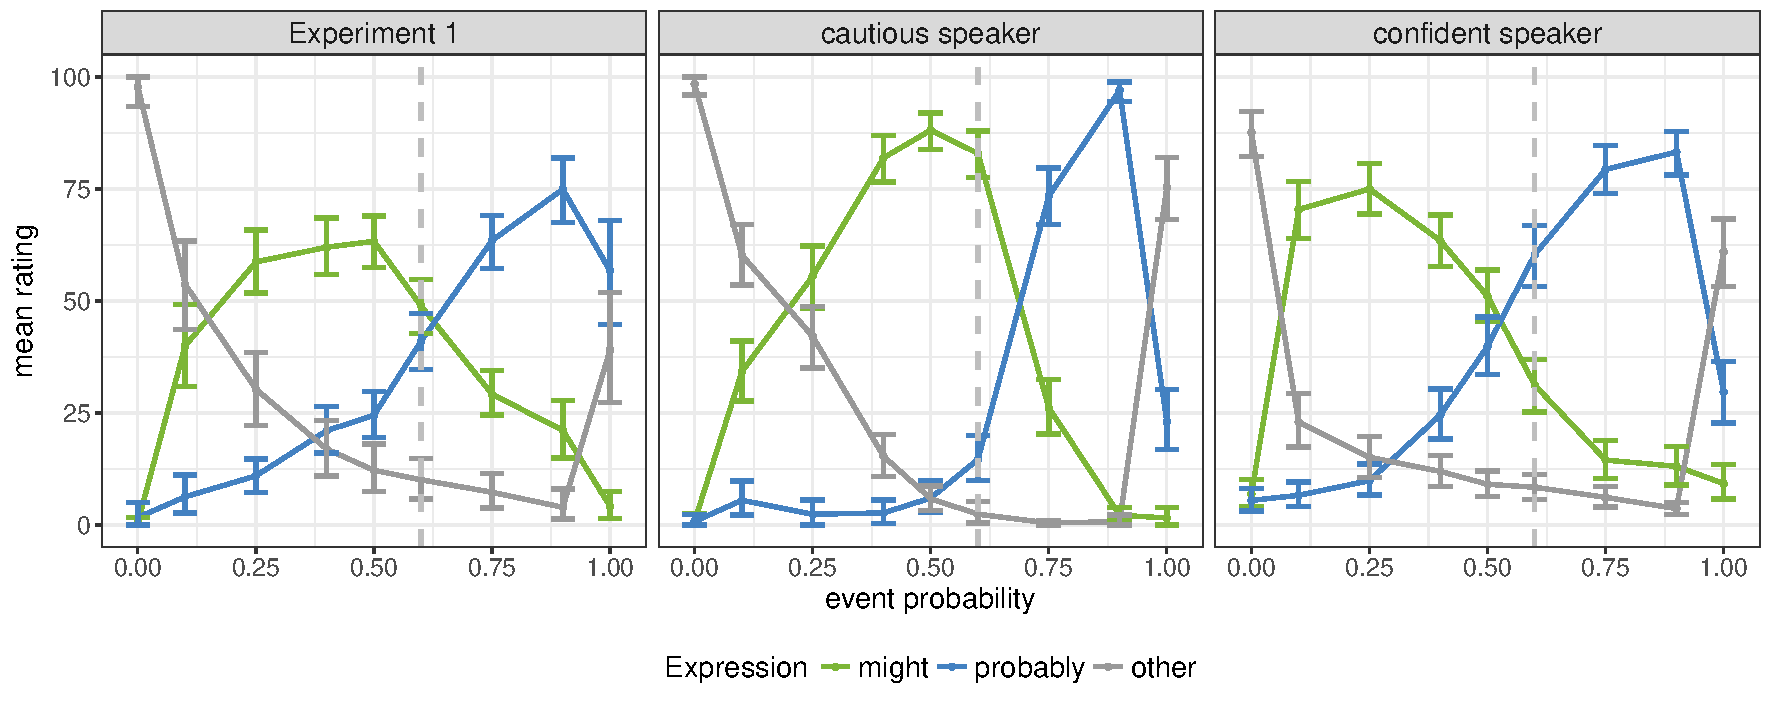
\includegraphics[width=\textwidth]{plots/fig-8-exp-1-replication-ratings.pdf}
\caption{Mean ratings for the \textit{might-probably} condition from Experiment 1 (repeated from \figref{fig:norming-results-main}) and mean post-exposure ratings from Experiment~2. Error bars correspond to bootstrapped 95\%-confidence intervals.  The grey dotted line highlights the ratings for the 60\% event probability ratings.  \label{fig:adaptation-results-prod}}
\end{figure}

% Figure 9: plots/fig-9-exp-1-auc.pdf (1-column figure)
\begin{figure}
\center
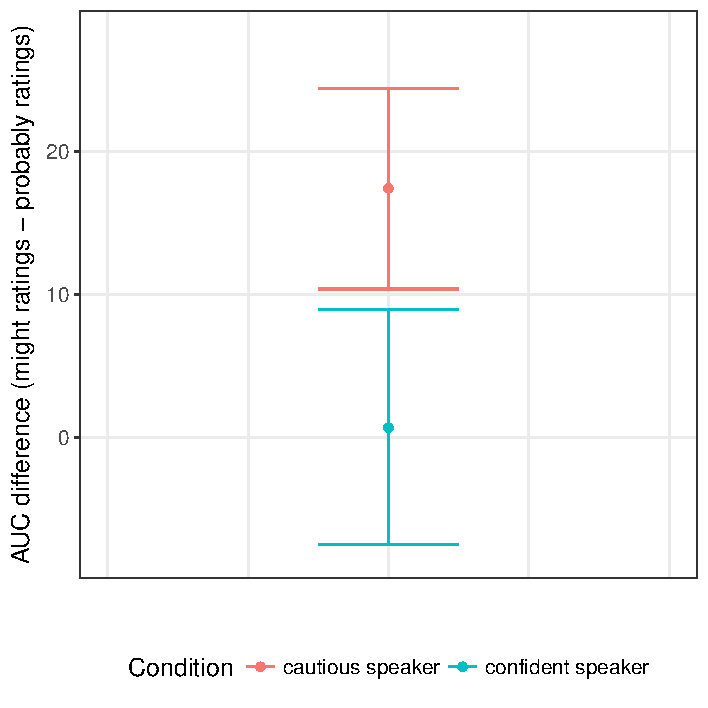
\includegraphics[width=.4\textwidth]{plots/fig-9-exp-1-auc.pdf}
\caption{Area under the curve (AUC) differences from Experiment~2. Error bars correspond to bootstrapped 95\%-confidence intervals.  \label{fig:adaptation-auc-prod}}
\end{figure}

The center and right panels of Figure~\ref{fig:adaptation-results-prod} show the mean ratings for the three options in the two conditions. As these plots show, participants updated their expectations about the speaker's language use, and therefore made different predictions about how the speaker would use uncertainty expressions as compared to prior expectations elicited in Experiment~1 (left panel). In the \emph{cautious speaker} condition, participants gave high ratings for {\sc might} for a larger range of event probabilities than in the \emph{confident speaker} condition. On the other hand, participants gave high ratings for {\sc probably} for a larger range of gumball proportions in the \emph{confident speaker} condition than in the \emph{cautious speaker} condition. These differences result in a significantly larger AUC difference in the \emph{cautious speaker} condition than in the \emph{confident speaker} condition ($t(63) = 2.99$, $p < 0.01$, see also Figure~\ref{fig:adaptation-auc-prod}).

As Figure~\ref{fig:adaptation-results-prod} shows, participants also differed in their ratings of the two utterances when they were presented with a scene with 60\% target color gumballs. In Experiment~1, participants assigned approximately equal ratings to both expressions; in the \emph{cautious speaker} condition, participants rated {\sc might} higher than {\sc probably}; in the \emph{confident speaker} condition, the pattern was reversed and participants rated {\sc probably} higher than {\sc might}. These expectations mirror the speaker behavior during the exposure phase and provide additional evidence that participants tracked the speaker's usage of uncertainty expressions. 

The results further suggest that participants updated their mappings between uncertainty expressions and event probabilities: In the {\it confident speaker} condition, {\sc might} and {\sc probably} were rated highly for lower event probabilities than in the {\it cautious speaker} condition. This experiment further provides evidence against an account according to which participants only learn that the \emph{cautious speaker} prefers to use {\sc might} and the {\it confident speaker} prefers {\sc probably}. Since the frequency of both expressions was the same in this experiment, participants could not have inferred a preference for one of these two utterances. 

In sum, the results from this experiment provide evidence for listener adaptation to a specific speaker's use of uncertainty expressions after a brief exposure phase. Further, the results 
suggest that listeners' expectations about a speaker's language use are at least not exclusively driven by tracking speakers' preferences for different utterances. We investigate the nature of the updated expectations
in the next section.


\section{Adaptation model}
\label{sec:model-adapt}



The experimental results presented in the previous section suggest that listeners update
\textit{some} expectations about language use when they interact with a speaker. 
However, the nature of the updated representations is unclear. As mentioned in the introduction, there are three likely candidates:
first, it is possible that listeners update their expectations about the speaker's lexicon 
(i.e., the mapping between event probabilities and uncertainty expressions);  second, listeners
 might  update their expectations about the speaker's preferences; 
and third, they might update both their expectations about the speaker's lexicon 
and about the speaker's preferences. The experimental results above suggest that it is unlikely that listeners track only speaker preferences, but considering
that beliefs about preferences and beliefs about the lexicon can interact in complex ways (as illustrated in \figref{fig:inference-example}), we investigate all three options.

The production expectation model in \sectionref{sec:model-baseline} provides us with the opportunity to formally evaluate these three hypotheses.
Through a series of simulations of the adaptation process, we can compare models in which different types of parameters are
 updated during adaptation. Following work in modeling adaptation in other linguistic domains \cite[e.g.,][]{Kleinschmidt2012,Kleinschmidt2015,Qing2014,Hawkins2017,Roettger2019}, 
we assume that in interaction, listeners form beliefs about a set of speaker-specific parameters $\Theta_S$.\footnote{Since the manipulation in our experiments was between subjects, our results do not provide direct evidence that listeners are indeed adapting to speakers (as compared, for example, to the general experimental situation). For now, we assume that listeners are adapting to specific speakers and we return to this issue in the general discussion.
Further, the speaker-specific parameters might be correlated and  listeners might form beliefs about bundles of correlated parameters instead of forming beliefs about individual parameters. For simplicity, we assume here that individual parameters are independent but it would be interesting to investigate whether, for example, listeners who expect a speaker to use lower thresholds for \textit{probably} also expect the same speaker to have lower thresholds for \textit{might} (see also Section~\ref{subsec:adaptation-model-evaluation}).}
We further assume that the formation of these beliefs is an instance of Bayesian belief updating:
listeners start off with prior beliefs about $\Theta_S$ based on their general knowledge about 
language and subsequently update their beliefs about $\Theta_S$ with every utterance they hear. 
That is, after observing a series of productions $D={d_1, ..., d_n}$ where each $d_i$ is an 
utterance-event probability pair $d_i = (u_i, \phi_i)$, listeners' beliefs about $\Theta_S$ are the result
of performing Bayesian inference:
$$P(\Theta_S \mid D) \propto P(\Theta_S) P(D \mid \Theta_S) = P(\Theta_S) \prod_{i=1}^nP(d_i \mid \Theta_S) $$

\noindent We assume that the likelihood function is the \textit{expected pragmatic speaker} $ES_1$ parameterized by $\Theta_S$:

$$P(\Theta_S \mid D) \propto P(\Theta_S)  \prod_{i=1}^n ES_1(u_i \mid \phi_i, \Theta_S) $$



\subsection{Simulations}

In order to investigate which parameters are updated during adaptation, we ran simulations
with varying prior structures, which correspond to different assumptions about which parameters may be updated.
The adaptation model crucially relies on a prior over speaker-specific parameters $P(\Theta_S)$
which reflects listeners' prior beliefs about the use of uncertainty expressions. For our simulations,
we assumed that the means of this prior are given by the estimates of the model parameters that 
we obtained from fitting the model to the norming data. The variances reflect whether or not the parameter can be updated in response to exposure. In particular, we used delta distributions, i.e., distributions with zero variance, to model a parameter that cannot be updated. We ran simulations on models with the following three prior structures:


\begin{itemize}
\item \textbf{\textit{Costs}}: The first prior structure corresponds to an adaptation process according to which participants only learn speaker preferences during adaptation. 
We modeled the prior over cost parameters  as a log-normal distribution centered at the mean value inferred from the norming data. Because we were interested in whether listeners update their beliefs about speaker preferences, we relaxed the assumption from the norming data model that all utterances have the same cost and assumed that each expression has its own cost parameter indicating beliefs about the speaker's preferences.\footnote{Note that since all updates of parameters happen as part of the belief updating simulations and we are not fitting model parameters to post-exposure ratings, we do not have to be concerned about overfitting due to too many parameters.} Use of the log-normal distribution was motivated by two reasons: First, cost must be greater than zero, and the support of log-normal distributions is limited to numbers greater than 0. Second, since the cost term is part of an exponent in the expected pragmatic speaker model, differences on a logarithmic scale correspond to linear differences in the model's utterance probabilities. For the priors over all other parameters, we used a delta distribution.
\item \textbf{\textit{Threshold distributions}}:  This prior structure corresponds to an adaptation process according to which participants only learn speaker-specific threshold distributions during adaptation. We parameterized threshold Beta distributions $P(\theta_e)$ with their mean $\mu_e$ and population parameter $\nu_e$ \cite{Kruschke2015}. Since the threshold and therefore also the mean of the threshold distribution have to lie within the interval [0,1], we used a truncated normal distribution $\mathscr{N}_{[0,1]}$, which we centered at the mean value from the norming data. For the population parameters $\nu_e$, which indicate how peaked a threshold distribution is, we assumed that distributions can only become more peaked when listeners are exposed to a speaker with very consistent language use and therefore modeled the prior as an exponential distribution shifted to the mean population parameter that we estimated from the norming data. We used a delta distribution for the priors over all other parameters.
\item  \textbf{\textit{Threshold distributions and costs}}:   This prior structure corresponds to an adaptation process according to which participants learn both speaker-specific threshold distributions and speaker preferences during adaptation.  We used the log-normal distributions as priors over the cost parameters and the truncated normal and exponential distributions as priors over the threshold distribution parameters, as described above. This means that both the threshold distributions and the cost parameters could be updated during the adaptation simulations.
\end{itemize}

Each of these prior structures corresponds to a different hypothesis about which expectations listeners update during adaptation. For comparison, we also considered a baseline in which none of the parameters are updated during adaptation (the {\it fixed} prior structure). To adjudicate between these three hypotheses, we ran simulations of the adaptation process for both (\textit{cautious speaker} and \textit{confident speaker}) conditions with different prior structures and compared the models in terms of their likelihood of generating the experimental data. During each simulation, we performed Bayesian inference to infer the posterior parameter distribution after observing the 25 data points that participants observed in the exposure phase (see Table~\ref{tbl:materials} for an overview of the 25 utterances in the two conditions). We performed inference using MCMC with a Metropolis-Hastings sampler. We used thinning of 10, discarded the first 2,000 burn-in samples and collected 10,000 samples from each of the two chains.

% Table 4
\begin{table}
\center
\begin{tabular}{l | c | c | c  }
 & Range &  Step size & MAP value  \\ \midrule
Variance for $\mu$ & [0.025,0.25] & 0.025 & 0.175  \\
Scale for $\nu$  & [0.5,4.5]  & 0.5   & 3.5  \\
Variance for cost & [0.1,1.5] & 0.2 & 0.7  \\
\end{tabular}
\caption{Explored hyperparameter ranges for variance parameters, and inferred MAP values, which were used in the adaptation simulations.  \label{tbl:hyperparams}}
\end{table}


The prior distributions over the different parameters that may be updated during the adaptation simulations are all parameterized by two constants which govern their mean and their variance. The first set of parameters (the mean of the log-normal and truncated normal distributions; the location parameter of the exponential distributions) was given by the estimates from fitting the model to the norming data. The second set of parameters (the variance of the log-normal and truncated normal distributions; the scale parameter of the exponential distributions) was treated as hyperparameters of the simulations. To keep the model as simple as possible, we only used three hyperparameters in total: a variance parameter for the cost for all expressions; a variance parameter for the mean of the threshold distributions for all utterances; and a scale parameter for the prior over population parameters for all utterances. We optimized these three parameters through a Bayesian hyperparameter search on the adaptation data, which provided us with a distribution over hyperparameter values. Considering that each simulation is computationally expensive, we could only test a few hundred hyperparameter combinations, which are listed in Table~\ref{tbl:hyperparams}. We found that the resulting distributions were highly peaked and therefore, we used only the maximum a posteriori estimates of the hyperparameters (also shown in Table~\ref{tbl:hyperparams}) for the model comparisons below.


\subsection{Model comparisons}

We compared model fits via the likelihood of the model generating the post-exposure data. To compute this metric, we constructed a dataset $D_{obs}$ of utterance-event probability pairs by treating each post-exposure rating as a probability distribution and sampling 10 utterances from it. We then computed the posterior likelihood odds between Model 1 with posterior distribution over parameters $P(\Theta_{S}^{(1)})$ and Model 2 with posterior distribution $P(\Theta_{S}^{(2)})$.

$$\mbox{posterior likelihood odds} = \frac{\mathlarger{\int_{0}^{1}} {P\left(\Theta_{S}^{(1)}\right) P\left(D_{obs} \mid \Theta_{S}^{(1)} \right) d   \Theta_{S}^{(1)}}}{\mathlarger{\int_0^1} P\left(\Theta_{S}^{(2)}\right) P\left(D_{obs} \mid \Theta_{S}^{(2)}\right)d   \Theta_{S}^{(2)} }$$
 
\noindent The posterior likelihood odds indicate how much more likely it is that the data was generated by Model 1 than by Model 2. Note that we are marginalizing over distributions over parameter values (the integrals in the above formula) and the more parameters we allow to update, the more dispersed the distributions over parameters  $P\left(\Theta_{S}^{(1)}\right)$ and $P\left(\Theta_{S}^{(2)}\right)$ will be. At the same time, the likelihood terms $P\left(D_{obs} \mid \Theta_{S}^{(1)}\right)$ and $P\left(D_{obs} \mid \Theta_{S}^{(2)}\right)$ will only be high for a small range of parameter assignments. Taken together, this means that the posterior odds metric will naturally favor simpler models, because the more dispersed the distributions over parameters are, the less weight is assigned to parameter configurations that yield a high likelihood of generating the data \cite[a property often referred to as Bayesian Occam's razor; see, e.g., ][]{MacKay1992,Neal1995}. 

To evaluate how well the different models predict the empirical post-exposure ratings, we also compute the $R^2$ value between participants' average 
post-exposure ratings and the maximum a posteriori predictions of the post-exposure model. However, while $R^2$ values close to 1 always indicate 
that model predictions closely match empirical ratings, it is important to note that there are multiple caveats with using $R^2$ in our setup. 
First, $R^2$ is based on the assumption that all predictions are independent and that the residual error follows a normal distribution. 
These assumptions generally hold for regression models but they are violated for our model predictions since the model predicts a 
probability distribution over utterances for each event likelihood and therefore predicted utterance ratings are not independent and the 
residual errors do not follow a normal distribution. Further, unlike the posterior odds,
$R^2$ does not take uncertainty of the model predictions into account but instead compares the mean participant behavior to the mean 
model predictions, and therefore is not a well-suited measure for comparing models exhibiting uncertainty.\footnote{If the assumptions of independence and normally distributed 
residual errors were met, we could address the issue of uncertain model predictions by using a recently proposed Bayesian $R^2$ metric \cite{Gelman2019}, 
which takes uncertainty of model predictions into account and returns a distribution over $R^2$ values. 
However, the computation of this metric crucially relies on estimates of the variance of the residual error $\sigma^2$, and it neither 
makes sense nor is possible in our current framework to estimate this quantity. Hence, we also cannot compute a meaningful Bayesian $R^2$ distribution.} 
For these reasons, we present $R^2$ values only to provide intuitions about how well the model predictions match the empirical ratings. For the formal model comparisons we 
rely on the posterior odds.\footnote{For all simulations discussed in this and following sections, we find that the $R^2$ and the posterior odds lead to the same conclusions but in an additional simulation experiment, reported in Appendix~F, we encountered a case where the two metrics disagreed.} 

% Table 5
\begin{table}
\center
\begin{tabular}{r | c | c }
Model &   odds  &  $R^2$ \\ \midrule
fixed & $10^{-1265}$ &  0.673       \\
cost & $10^{-478}$ & 0.817     \\
threshold distributions & $10^{-187}$ &  0.885 \\
cost \& threshold distributions & 1 &  0.901 \\
\end{tabular}
\caption{Model evaluation results on data from Experiment~2.   \textit{odds} are the posterior likelihood odds of the models compared to the \textit{cost and threshold distributions} model.  $R$\textsuperscript{$2$} are computed between  the mean post-exposure ratings and the mean model predictions. \label{tbl:model-comparison-replication}}
\end{table}

Table~\ref{tbl:model-comparison-replication} shows 
the posterior likelihood odds and the $R^2$ values between the the models and the experimental data from Experiment 2. 
As the values in this table show, the model in which the cost as well as the threshold 
distributions are updated during adaptation is much more likely to generate the experimental data than the other two adaptation models
as well as the prior model. Further, this model closely predicts participants post-exposure behavior, as indicated by the high $R^2$ value. 
 
 
What do these modeling results tell us about the semantic/pragmatic adaptation process? 
We assumed that each of these simulations
correspond to an adaptation process in which different types of expectations are  updated.
The modeling results corroborate the experimental results from Experiment~2:
the models according to which no expectations are updated during adaptation (the \textit{fixed} model) 
or according to which only preferences are updated (the \textit{cost} model) provide poor predictions for the post-adaptation
ratings. The results further clearly indicate that listeners update expectations about the threshold distributions: The two models according to 
which listeners update threshold distributions were best at predicting post-adaptation behavior. Overall, however, the model that allows updating
of preferences and threshold distributions (the \textit{cost \& threshold distributions} model) provides the best predictions of post-adaptation ratings, which
provides evidence that listeners update expectations about both {threshold distributions} and {preferences}. 


\subsection{Model evaluation}
\label{subsec:adaptation-model-evaluation}

% Figure 10: plots/fig-10-adaptation-posterior-predictions-replication.pdf  (2-column figure)
\begin{figure}
  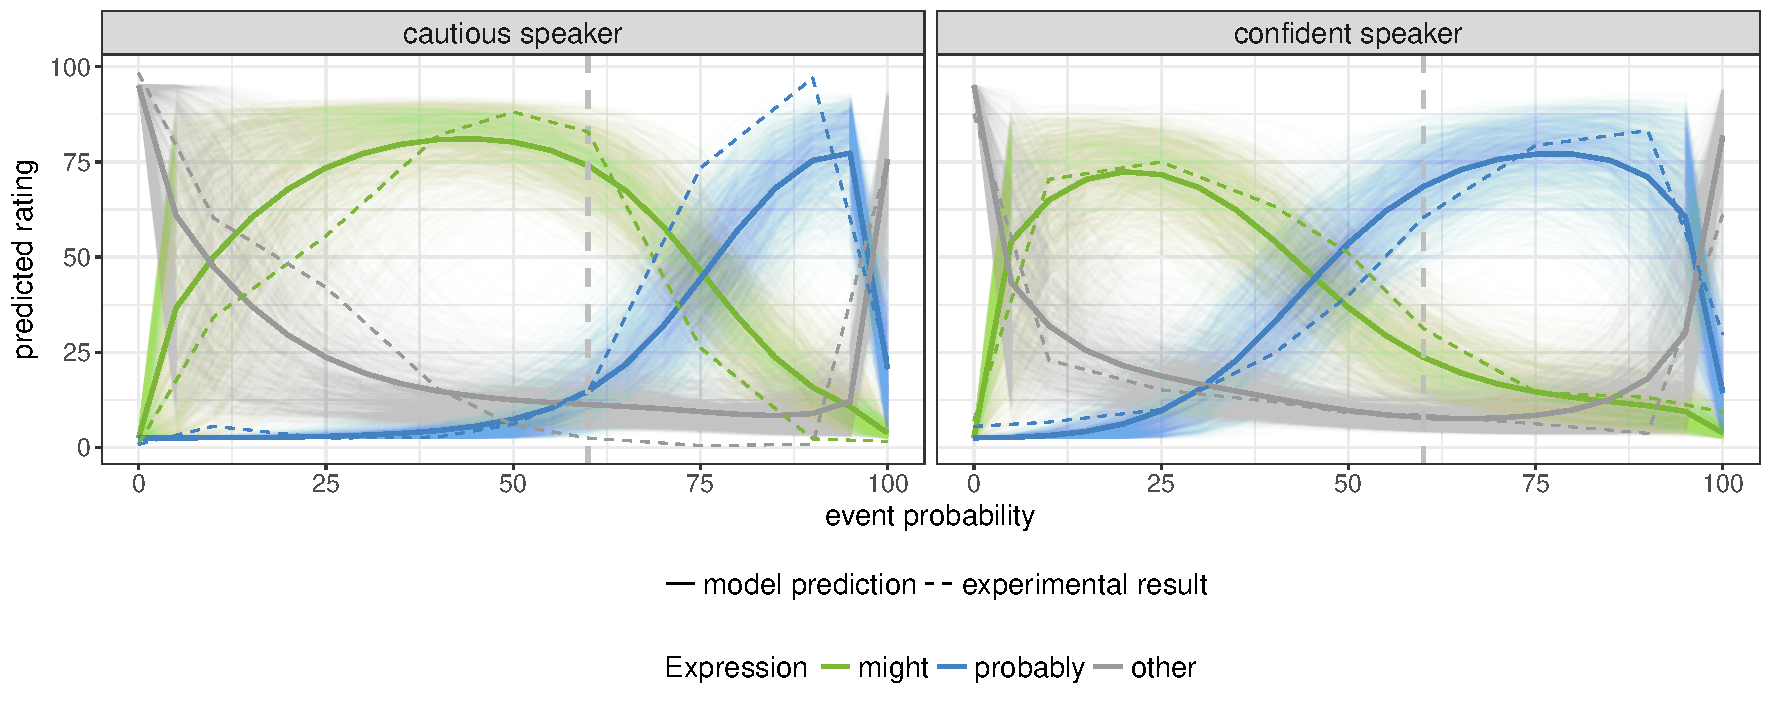
\includegraphics[width=\textwidth]{plots/fig-10-adaptation-posterior-predictions-replication.pdf}
  \caption{Post-adaptation model predictions from simulations for Experiment~2 and experimental results. 
  The solid lines shows the mean model predictions and the thin lines around the mean show the distribution of model predictions. \label{fig:post-exposure-model}}
\end{figure}

Apart from quantitatively assessing the fit of the model, it is informative to visually inspect the predictions of the model to verify that the model makes correct qualitative predictions. 
Figure~\ref{fig:post-exposure-model} shows the post-exposure predictions of the \textit{cost \& threshold distributions} model compared to the average participant ratings for the two conditions from Experiment~2.
Qualitatively, 
the model captures several important patterns in the post-adaptation behavior. The model correctly predicts that in the \textit{cautious speaker} condition, ratings for \textsc{might} are 
higher than ratings for \textsc{probably} when there is an objective probability of 0.6. For the \textit{confident speaker} condition, the model correctly predicts the
opposite pattern. The model also predicts that in the \textit{cautious speaker} condition, participants rate \textsc{might} highly for a larger range of event probabilities than
in the \textit{confident speaker} condition and the model predicts the  reverse pattern for the \textsc{probably} ratings. Further, the model predicts that high ratings for \textsc{might} 
and \textsc{probably} are not limited to the utterance-event probability combinations that participants observed during the exposure phase. For example, the model correctly predicts
high ratings of \textsc{might} for low event probabilities in the \textit{cautious speaker} condition despite the fact that it never observed utterances for low event probabilities. Similarly,
the model predicts high rating of \textsc{probably} for high event probabilities in the \textit{confident speaker} condition -- a combination which was again not part of the exposure trials
of this condition.

Quantitatively, there are some differences between the model predictions and participant behavior. This is not surprising considering that the model predictions are a result of simulations
and, with the exception of the three variance parameters of the prior distributions, we did not fit any model parameters to the behavioral data. One difference is that the model underpredicts 
the ratings of one of the  \textsc{probably} utterances in the \textit{cautious speaker} condition.
 One reason for this deviation could be the relatively simple prior structure. For the priors, we made the assumption that all model parameters are independent of each other and 
that the variance for the different parameter types is the same for all utterances. However, it could be that listeners have more structured prior beliefs such that priors over different parameters are correlated or
variances of prior distributions differ. For example, it could be that listeners expect the thresholds for \textit{might} and \textit{probably} to be correlated such that higher thresholds for \textit{might} are correlated 
with higher thresholds for \textit{probably}. Or it could be that listeners expect more between-speaker variation for some expressions than for others. Considering that we only have data from two experiments to test
model predictions and therefore would likely overfit to the data if we tried to fit more complex prior structures with more parameters, we leave the investigation of the exact structure of listeners' prior beliefs to future work.

% Figure 11: plots/fig-11-adaptation-posterior-thresholds-replication.pdf  (1.5-column figure)
\begin{figure}
  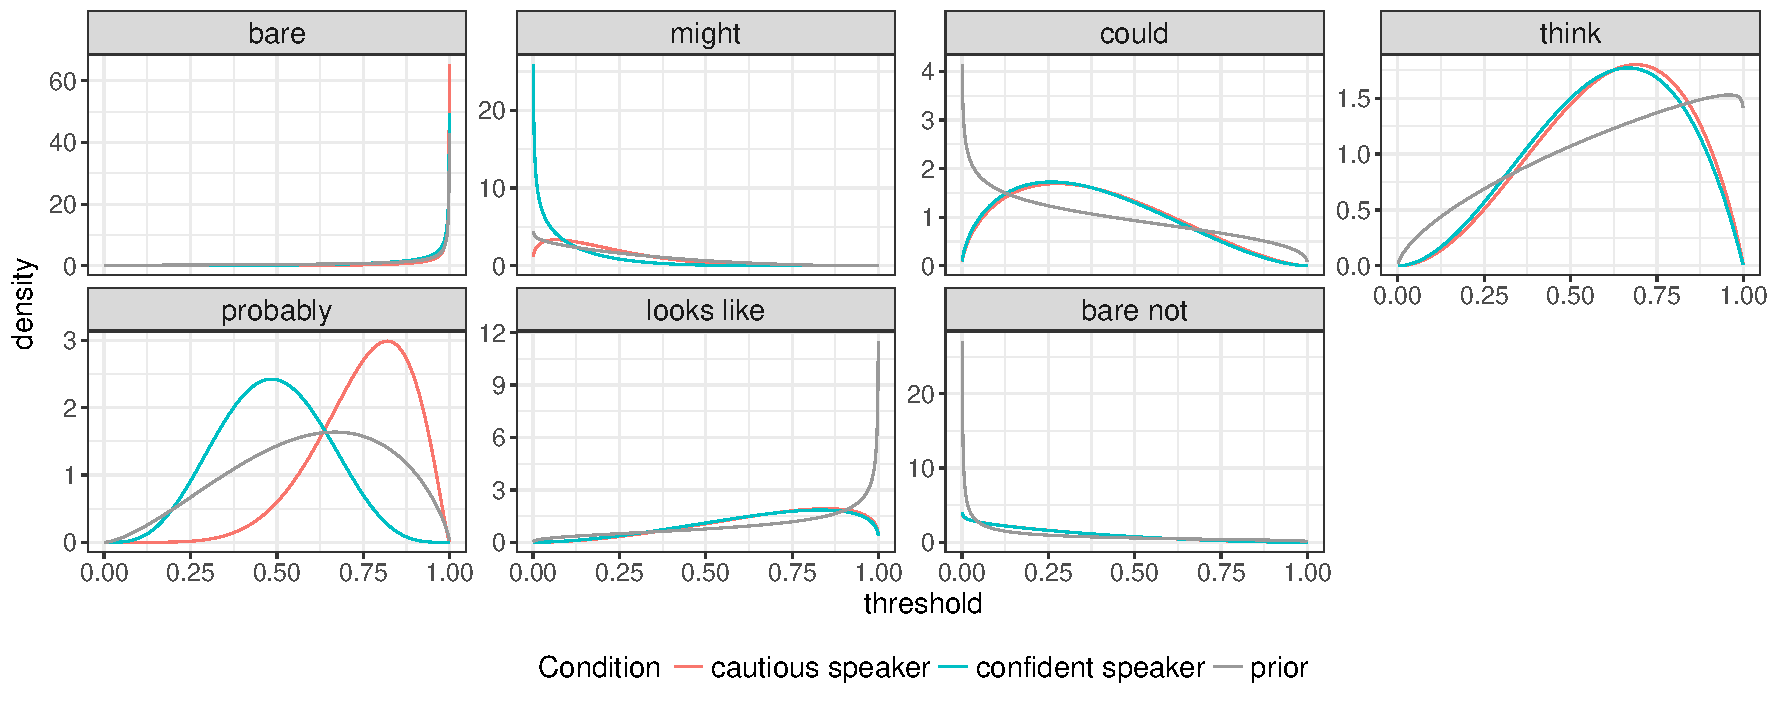
\includegraphics[width=\textwidth]{plots/fig-11-adaptation-posterior-thresholds-replication.pdf}
  \caption{Post-adaptation threshold distributions from the simulations for Experiment~2. \label{fig:post-exposure-thresholds}}
\end{figure}




The second noticeable deviation is that in the \textit{confident speaker} condition, the model overpredicts the ratings of the \textsc{other} utterance for event probabilities of 1 . This prediction is primarily driven by high values for the predicted ratings of \textsc{bare}. However, we argue that the model predictions in this case are reasonable, and that the lower participant ratings are likely an artifact of the experimental task. After completing the experiment, 
several participants indicated in a feedback form that they were confused by the lack of an option to rate the \textsc{bare} utterance, 
which they had heard during the exposure phase. In light of this confusion, almost all individual participants chose among two strategies when there was an event probability of 1: they either provided a rating of 100 for \textsc{other} 
or they provided a rating of 100 for \textsc{probably}, which on average leads to the ratings shown in \figref{fig:post-exposure-model}.

With the exception of these two deviations, the model makes not only correct qualitative, but also accurate quantitative predictions for the post-exposure ratings.

Lastly, we can also inspect how the model arrived at its predictions by looking at the inferred model parameters.  
Figures~\ref{fig:post-exposure-thresholds} and \ref{fig:post-exposure-costs} show the inferred
post-exposure threshold distributions and costs for the two conditions as well as the distributions inferred from the norming data.
Figure~\ref{fig:post-exposure-thresholds} shows that the threshold distribution for \textit{probably}
changed considerably depending on the exposure phase: in the \textit{cautious speaker} condition,
its mean shifted to a higher value than  inferred from the norming data; in the \textit{confident speaker} condition the mean 
shifted to a lower value. To a lesser extent, we observe similar shifts in the mean of the threshold
distributions for \textit{might}. We further observe that for all expressions, the variance of the threshold
distributions decreased as a result of adaptation. In the case of the expressions that were part of the exposure
phase, this is expected, since the exposure speaker used these expressions very consistently; in the case of the
other expressions, this decrease in variance is a result of the exponential prior over the population parameter,
which biased the model towards lower variance. For some of the thresholds, this resulted in differently shaped distributions.
However, note that the area under the curve of all threshold distributions except for \textit{probably} is still very similar to the 
area under the curve of the norming data threshold distributions. And overall, except for the distributions
for \textit{might} and \textit{probably}, the post-exposure threshold distributions are almost identical in both conditions.
This suggests that the post-adaptation expectations 
are in part a result of updated threshold distributions for \textit{might} and \textit{probably}.

% Figure 12: plots/fig-12-adaptation-posterior-costs-replication.pdf  (1-column figure)
\begin{figure}
\center
  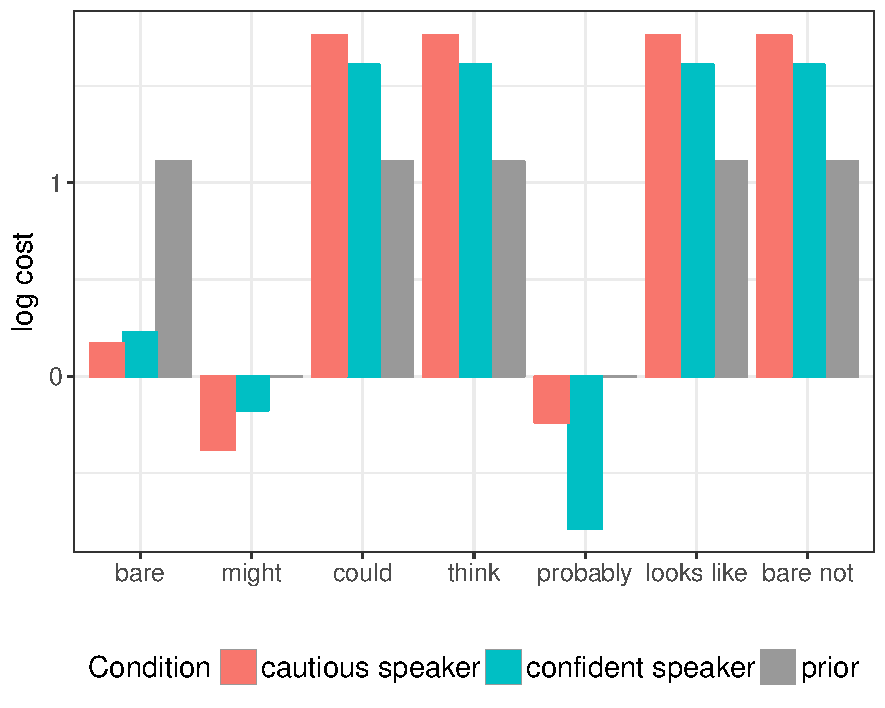
\includegraphics[width=0.5\textwidth]{plots/fig-12-adaptation-posterior-costs-replication.pdf}
  \caption{Post-adaptation $log$ cost values from simulations for Experiment~2. Note that the cost of \textsc{might} and \textsc{probably} 
  in the norming data model was 1 and therefore the $log$ cost for these utterances is 0. \label{fig:post-exposure-costs}}
\end{figure}

Figure~\ref{fig:post-exposure-costs} shows that the costs of the \textsc{might}, \textsc{probably} and
\textsc{bare} utterances, i.e., the three utterances that participants observed during the exposure phase,
all decreased while the costs of the other four utterances increased compared to the costs inferred from the norming
data. Further, the post-exposure cost of \textit{might} is lower than the cost of \textit{probably} in the \textit{cautious speaker} condition
and the opposite relation between these costs holds in the \textit{confident speaker} condition, which suggests that
that the post-adaptation expectations are in part also a result of updated beliefs about preferences of \textsc{might} and \textsc{probably}. 
This finding also highlights the complex interplay between threshold distributions and preferences: The number of exposure trials 
with \textsc{might} and \textsc{probably} was identical in both conditions, so participants could not have inferred a preference
based on exposure frequencies. Instead, participants seemed to indirectly infer that the \textit{cautious speaker} prefers to use \textsc{might} from the speaker's uses of \textsc{might} to describe a
larger range of event probabilities and that the \textit{confident speaker} prefers to use \textsc{probably} from the speaker's uses of \textsc{probably} for a
larger range of event probabilities. However, frequency nevertheless has an effect on inferred preferences. As shown in Appendix~F, the difference in inferred preferences 
was larger when participants in the \textit{cautious speaker} condition were exposed to more trials with \textsc{might} than in the \textit{confident speaker} condition and participants in the \textit{confident speaker} condition were exposed to more trials with \textsc{probably} than in the \textit{cautious speaker} condition.

\subsection{Interim summary}

In the previous two sections, we presented the results from an experiment that provides strong evidence for
listeners updating expectations about a speaker's use of uncertainty expressions after brief
exposure to that speaker. We further presented a computational adaptation model which models the adaptation
process as an instance of Bayesian belief updating. Using different implementations
of that model to investigate which kind of expectations listeners update during adaptation, we found strong evidence that listeners update beliefs both about  threshold distributions and 
 about speaker preferences.

% Section 6
\section{Experiment 3: Effect of adaptation on interpretation}
\label{sec:exp-model-interpretation}


Up to this point, we focused on listeners' expectations about a speaker's use of uncertainty expressions. As we discussed
in the introduction, we expect updated expectations to also have an effect on the \emph{interpretation} of uncertainty expressions. This
effect is also predicted by RSA models,  which assume that a pragmatic listener $L_1$ tries to infer the state of the world (in our case, the event probability $\phi$) by reasoning
about their prior beliefs about the world state and their expectations about a speaker's language use (in our case, the expected pragmatic speaker $ES_{1}$) via Bayes' rule:

$$ L_1(\phi \mid u_e) \propto P(\phi) ES_1(u_e \mid \phi).$$

According to such a model of interpretation, the shifts in expectations that we observed in the previous experiment should also lead to a shift in interpretations. 
If we assume a uniform prior over event probabilities,\footnote{To reiterate, this assumption was motivated by the study reported in Footnote 9, which suggested that participants on average assign equal probability to each gumball machine a priori. In this special case, we expect interpretations to be an exact mirror image of production expectations but in many other scenarios, listeners will have skewed prior beliefs about the event likelihood (e.g., consider beliefs about the likelihood of rain on a specific summer day in California, which will be highly skewed towards low values) and in such scenarios, listeners integrate prior beliefs and  production expectations to arrive at interpretations.} then the model predicts that listeners who were exposed to a \textit{cautious} speaker should infer 
higher event probabilities when hearing {\sc might} or {\sc probably} than listeners who were exposed to a \textit{confident} speaker. Figure~\ref{fig:post-exposure-comp}
shows the distribution over event probabilities after hearing three different utterances as predicted by $L_1$ parameterized by the inferred parameters from our
adaptation simulations in the previous section. As these plots show, in the \textit{cautious speaker} condition, the distribution over event probabilities after hearing \textit{might} 
and \textit{probably} is shifted towards higher values as compared to the distributions in the \textit{confident speaker} condition. 

% Figure 13: plots/fig-13-adaptation-posterior-comp.pdf  (2-column figure)
\begin{figure}
  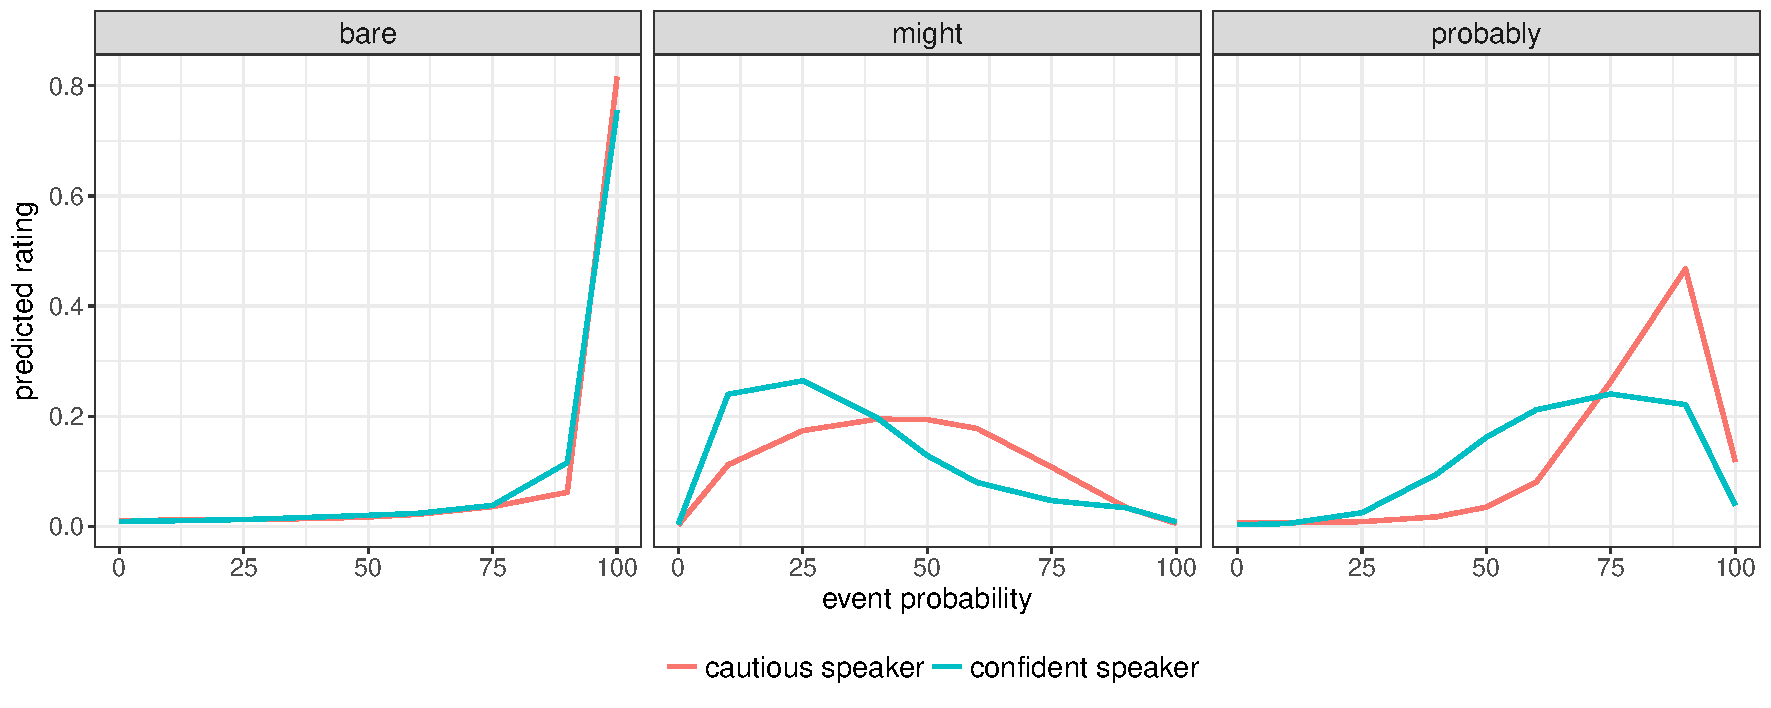
\includegraphics[width=\textwidth]{plots/fig-13-adaptation-posterior-comp.pdf}
  \caption{Post-adaptation interpretation distributions for the utterances  \textsc{bare}, \textsc{might}, and \textsc{probably} as predicted by the pragmatic listener $L$\textsubscript{$1$}. \label{fig:post-exposure-comp}}
\end{figure}

In this experiment, we tested whether this prediction is correct and whether listeners' change in expectations transfers to a change in interpretations. 
The procedure, materials and analyses were pre-registered at \url{https://osf.io/ghnc3}.\footnote{This experiment is a modified version of a previous experiment, which qualitatively yielded the same results but seemed to confuse some participants. See Appendix~G for a discussion of the original experiment.}

\subsection{Method}

\subsubsection{Participants}

We recruited a total of 80 participants (40 per condition) on Amazon Mechanical Turk. We required participants to have a US-based IP address and a minimal approval rating of 95\%. Participants were paid \$1.5 which amounted to an hourly wage of approximately \$15. None of the participants had participated in any of the previous experiments. 

\subsubsection{Materials and Procedure}

Participants completed a set of exposure trials followed by a set of test trials. The exposure trials were identical to the exposure trials in Experiment~2. The test trials probed participants' interpretations of the utterances {\sc might}, {\sc probably} and {\sc bare}. On each test trial, participants listened to a recording of the speaker from the exposure phase producing {\sc might}, {\sc probably} and {\sc bare} and then participants were asked to rate for 9 gumball machines with the same proportions of blue and orange gumballs as in the previous experiments how likely they thought it was that the speaker saw each of these gumball machines by distributing coins.  Participants distributed 10 coins per trial and completed 6 trials in total  -- one for each expression-color pair. The exposure phase again contained  6 attention check as in the previous experiment. However, given the low attention check performance in the previous experiments, we modified the attention checks. Instead of asking participants whether they saw an X on the previous trial, we asked participants to choose the gumball machine that they had seen on the previous trial among two machines displayed in random order.

\subsubsection{Exclusions}

We excluded participants who failed more than 2 attention checks, which led to 1 exclusion in the \emph{cautious speaker} condition and 1 exclusion in the \emph{confident speaker} condition.


\subsubsection{Analysis and Predictions}

If participants update their expectations of a specific speaker's use of uncertainty expressions,  we expect them to interpret a more confident speaker's utterance 
to communicate a lower event probability than a more cautious speaker's utterance. We tested this prediction by treating participant's distributions of coins 
of gumball machines as a probability distribution over gumball proportions (and consequently event probabilities).  For each utterance, we 
normalized participants' coin distributions such that they summed up to 1, so that we could interpret the normalized scores 
as a categorical probability distribution over gumball machines given an utterance. We then compared the resulting distributions
over target color gumball proportions for each utterance in terms of their expected value, using a $t$-test.
 We predicted that the expected values of 
{\sc might} and {\sc probably} would be larger in the \emph{cautious speaker} condition than in the \emph{confident speaker} condition.

\subsection{Results and Discussion}

% Figure 14: plots/fig-14-exp-2-ratings.pdf  (2-column figure)
\begin{figure}
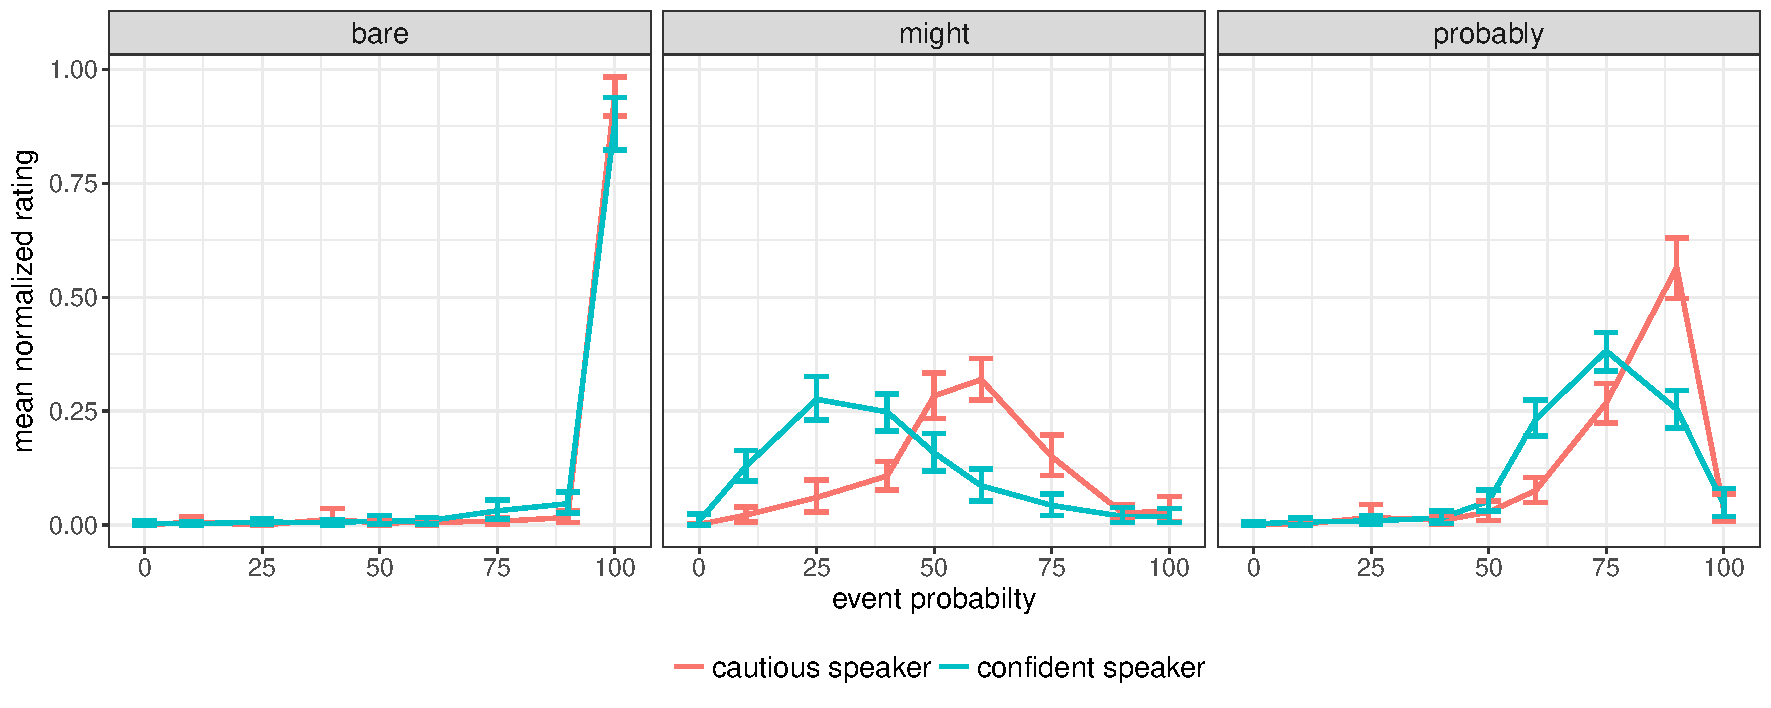
\includegraphics[width=\textwidth]{plots/fig-14-exp-2-ratings.pdf}
\caption{Aggregated post-exposure ratings from Experiment~3. Error bars correspond to bootstrapped 95\%-confidence intervals.  \label{fig:adaptation-results-comp}}
\end{figure}

Figure~\ref{fig:adaptation-results-comp} shows the aggregated and normalized ratings for the two conditions.  As predicted, participants provided higher ratings for gumball machines with higher target color percentages after hearing {\sc might} and {\sc probably} in the \emph{cautious speaker} condition than in the \emph{confident speaker} condition. This also led to a significantly higher expected value for {\sc might} ($t(76)=5.84$, $p<0.001$) and {\sc probably} ($t(76)=3.92$, $p<0.001$) in the \emph{cautious speaker} condition as compared to the \emph{confident speaker} condition.

These results suggest that listeners not only update their expectations about a speaker's use of uncertainty expressions, but also use those updated expectations in interpretation. 
Here, we made the implicit linking assumption that the distribution of coins reflects participants'  beliefs about event likelihoods after hearing an utterance.
The choice for this paradigm, which is very similar to betting paradigms that have been used to study utterance interpretation in reference games \cite{Frank2012,Goodman2013} as well as for probing subjective probabilities \cite[e.g.,][]{Hampton1973}, was motivated by the assumption that listeners will have uncertainty about the exact event likelihood after hearing \textsc{might} or \textsc{probably}. Allowing
participants to assign multiple coins to gumball machines with different proportions provided them with the ability to convey this uncertainty. The results from this experiment suggest that
participants behaved as expected: they assigned almost all coins to the gumball machine with 100\% target color gumballs after hearing \textsc{bare}, 
an utterance about whose interpretation participants likely have very little uncertainty, whereas they assigned coins to multiple machines after hearing \textsc{might} or \textsc{probably}. 


\subsection{Model comparison}

% Table 6
\begin{table}
\center
\begin{tabular}{r | c | c }
Model &   odds & $R^2$   \\ \midrule
fixed  & $10^{-452}$ & 0.827     \\
cost  &  $10^{-231}$ & 0.883       \\
threshold distributions  & $10^{-129}$ & 0.887 \\
cost \& threshold distributions & 1 &   0.936     \\
\end{tabular}
\caption{Model evaluation results on data from Experiment~3.  \textit{odds} are the posterior likelihood odds of the models compared to the \textit{cost and threshold distributions} model. $R$\textsuperscript{$2$} are computed between  the mean post-exposure ratings and the mean model predictions.  \label{tbl:model-comparison-comp}}
\end{table}



We return again to our main research question regarding which expectations are updated during adaptation. The production expectation experiments and model simulations provided strong evidence for listeners updating 
their beliefs about the threshold distributions and preferences. 
To determine the stability of these results, we also compared the pragmatic listener $L_1$ predictions from the simulations with different prior structures to the post-exposure ratings in Experiment~3. To this end, we computed the predictions of the $L_1$ model from the
posterior distributions over model parameters that we obtained through the simulations in the previous section. \tableref{tbl:model-comparison-comp} shows the model fit
for the different types of simulations. As this table shows, the model according to which both threshold distributions and costs are updated provides the best fit according to both metrics. 
Considering that the posterior likelihood odds consistently favored this model in all model comparisons, we take these results together as strong evidence that listeners update their expectations about threshold distributions
and costs. 

\subsection{Model evaluation}


\figref{fig:post-exposure-comp-data} superimposes the model predictions and the experimental data. As these plots show, the model accurately captures most of the qualitative and quantitative patterns. First, 
the model makes both qualitatively and quantitatively accurate predictions for the interpretation of the \textsc{bare} utterance in both conditions. Second, the model makes the crucial qualitative prediction that participants expect the speaker to communicate lower event probabilities in the \textit{confident speaker} condition than in the \textit{cautious speaker} condition, which we also observed in Experiment~3. Further, even though we used the parameters that we obtained in the simulations from the previous section and did not fit any parameters to the data from Experiment~3, the model also provides good quantitative predictions of participant's interpretation of \textsc{might} and \textsc{probably},
which provides further support for the hypothesis that semantic/pragmatic adaptation is an instance of Bayesian belief updating.

The main deviation between the model predictions and the experimental data lies in the interpretation of \textsc{might} in the \textit{cautious speaker} condition. For this interpretation, the model predicts a less peaked distribution than the empirical distribution.  One explanation for this deviation could be that participants are considering alternative uncertainty expressions (e.g., \textit{very unlikely}) that we did not include in the model.  However, since fine-tuning the set of alternative utterances would not change the qualitative predictions of the model and would not provide additional theoretical insights, we leave a more detailed exploration of this issue to future work. 

% Figure 15: plots/fig-15-adaptation-posterior-comp-data.pdf  (2-column figure)
\begin{figure}
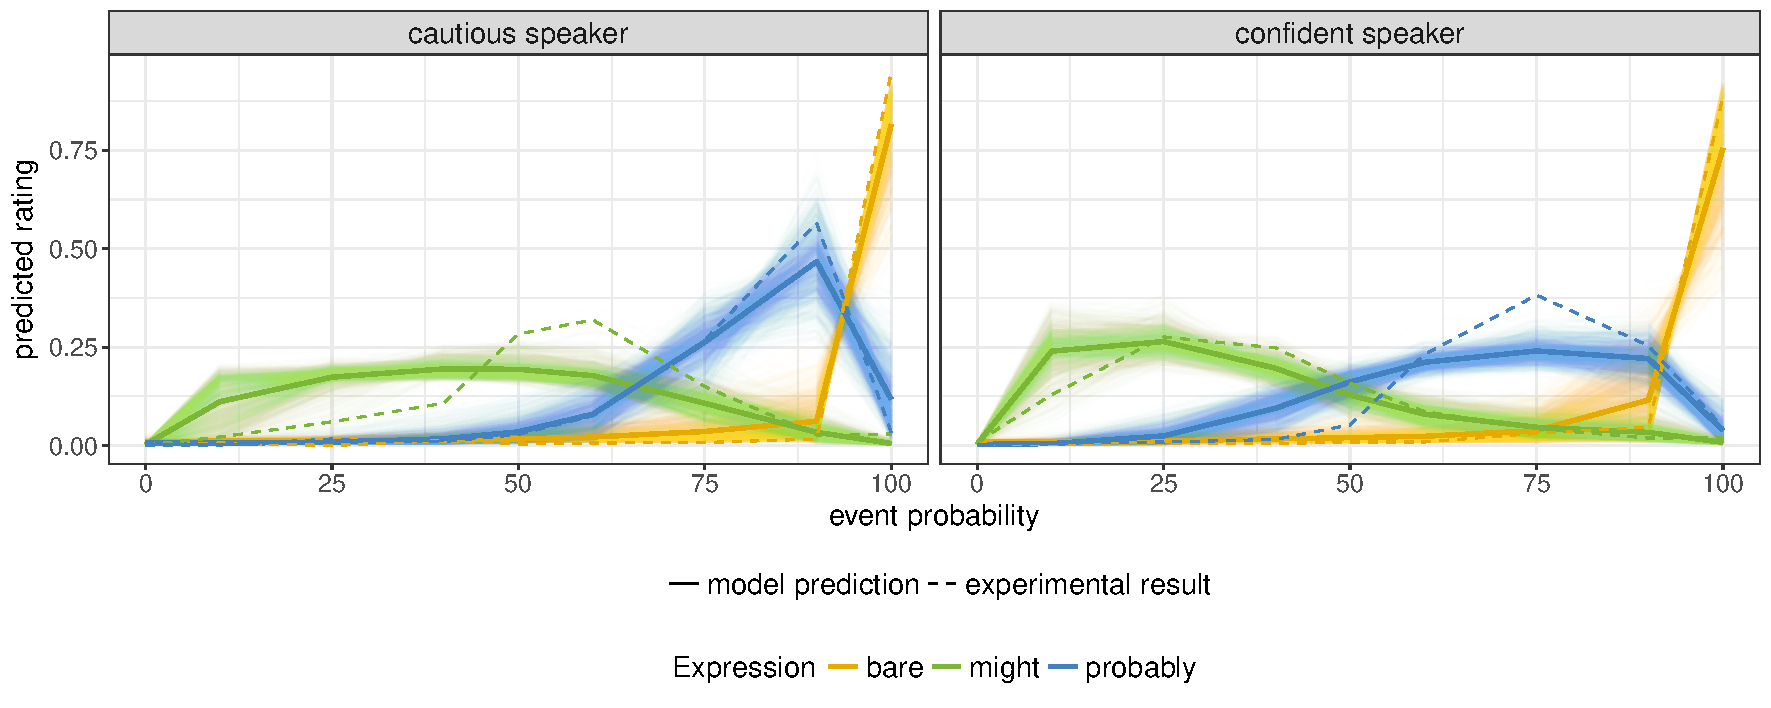
\includegraphics[width=\textwidth]{plots/fig-15-adaptation-posterior-comp-data.pdf}
\caption{Predictions of \textit{threshold distributions and costs} model and data from Experiment~3. The thin lines around the mean show the distribution of model predictions.  \label{fig:post-exposure-comp-data}}
\end{figure}


% Section 7
\section{General Discussion}

While adaptation in language is a widely attested phenomenon, the nature of the representations that are updated during semantic/pragmatic adaptation has largely remained a mystery. In this paper our contribution has been three-fold: 

First, in a production expectation experiment (Experiment~2), we showed that listeners adapt to speakers who vary in their use of uncertainty expressions, demonstrating that that 
the findings from \cite{Yildirim2016} extend to the class of uncertainty expressions. Second, we showed that updated \emph{production} expectations also affect subsequent utterance \emph{interpretation}  (Experiment~3). Finally, in a series of model comparisons, we found strong evidence for listeners updating their beliefs about both the speaker's lexicon as well as the speaker's preferences, which suggests
that semantic/pragmatic adaptation is a result of updating both of these representations. We further found that modeling the adaptation process as an instance of Bayesian
belief updating explains participants' post-adaptation behavior in both the production expectation (Experiments~2) and comprehension (Experiment~3) experiments. 

We next discuss the implications of this work for other accounts of adaptation and for semantic theories of uncertainty expressions, as well as its methodological implications. We then turn to limitations of the current results and account and discuss promising future research avenues this work opens. 


\subsection{Implications for and relation to other accounts of adaptation}

The model in this paper is formulated at the computational level \cite{Marr1982,Anderson1990} 
and is therefore directly only comparable to other computational models. However, we can still assess 
the compatibility of our findings with mechanistic accounts. We first discuss the relation to existing computational 
models of adaptation and then discuss what the results tell us about existing mechanistic accounts of
 adaptation.

The model presented above follows several other computational models of linguistic adaptation that are based 
on Bayesian belief updating, including models of phonetic adaptation \cite{Kleinschmidt2015}, syntactic 
adaptation \cite{Kleinschmidt2012}, adaptation in the interpretation of prosodic cues \cite{Roettger2019},
and adaptation to variable use of the quantifiers \textit{some} and \textit{many} \cite{Qing2014}. 
All of these models are based on the same Bayesian belief updating procedure according to which listeners integrate
their prior linguistic expectations and observed linguistic behavior to form updated expectations that facilitate comprehension.
This updating procedure is in line with recent proposals of a ``Bayesian brain'' \cite[e.g.,][]{Clark2013,Friston2010} which argue that
many cognitive and perceptual processes can be seen as an instance of integrating prior beliefs with observed signals from the environment.

Similarly, the formation of conceptual pacts \cite{Clark1986} --  alignment in the formation of referring expressions -- has been explained using a model  similar to the one we have proposed here \cite{Hawkins2017}. Hawkins et al.'s model is based on the assumption that speakers and listeners have uncertainty about the lexicon \cite[see also][]{Bergen2016} and that in interaction, speakers 
and listeners update their beliefs about the shared lexicon, akin to the updating of threshold distributions 
in our model. This further suggests that belief updating plays an important role in partner-specific language processing.

In the space of mechanistic accounts, \cite{Pickering2004} argued that a lot of partner-specific linguistic behavior
 can be explained as the result of priming, i.e., the automatic activation of linguistic representations when 
a speaker produces an utterance or a listener hears an utterance. Their account has the appeal
of explaining why partner-specific language use often appears to happen automatically and effortlessly. 
With the additional stipulation that the activated representations include information about both language
and the situational context and thus are able to represent variable semantics of uncertainty expressions,
their account appears to be compatible with our results. However, considering that \cite{Yildirim2016} and 
\cite{Schuster2019} found that listeners form speaker-specific expectations rather than expecting speakers
to behave like the most recent speaker they encountered, adaptation seems to be a more complex process than predicted by a
priming account.

In a more recent proposal, \cite{Pickering2013} agued that
at least sometimes listeners perform \textit{prediction-by-association} when processing
an utterance, that is, listeners make predictions about what the speaker would say based on
the context and their experience with the speaker.  This appears to
be compatible with our computational adaptation model but more details need to be
worked out about how such predictions operate at the implementational level \cite{Marr1982}.

In a second line of work, \cite{Horton2005,Horton2016} argued that partner-specific
language use can be explained by an episodic memory account \cite{Goldinger1998,Johnson1997,Pierrehumbert2001}.
According to this account, individual linguistic events are encoded together with
speaker information and the world state in memory, which results in speaker-specific
linguistic representations. This account is compatible with our findings, if we assume
that individual utterance-world state pairs are stored in memory together with the speaker's 
identity, and that some additional inference mechanism gives rise to the more complex
pragmatic behavior that we observed in our experiments.

\subsection{Implications for the semantics of uncertainty expressions}

Our results also have implications for semantic theories of uncertainty expressions.
The finding that listeners rapidly update their beliefs about semantic thresholds of uncertainty expressions
suggests that the semantics of these expressions is highly dynamic and context-sensitive. This is broadly compatible with 
theoretical accounts of probability operators \cite[a subset of uncertainty expressions; e.g.,][]{Yalcin2010} which 
state that the meanings of probability operators are highly dynamic and largely determined by the context. Our results
suggest that the meaning of uncertainty expressions is even more dynamic than predicted by these accounts. First, we show that this dynamicity 
extends to a broader set of uncertainty expressions than is typically considered (e.g., \textit{might}), as has been recently also argued by \cite{Lassiter2016}. 
Second, while these accounts generally assume 
that the main source of variability in interpretation is the probability of the event
embedded under the uncertainty expressions, we find that knowledge of speaker identity also  importantly contributes variability.

Dynamic and context-sensitive semantics have also been proposed for many other types of expressions.
For example, \cite{Clark1983} argued that speakers and listeners
are able to compute novel senses of nouns and verbs on the fly. Similarly, in the domain of gradable adjectives such as \textit{tall},
\cite{Kennedy2007} and many others have argued that the interpretation of these adjectives crucially depends on contextual
parameters. Considering the prevalence of dynamic meanings for so many other types of expression, it is therefore not 
surprising that the interpretation of uncertainty expressions also appears to be highly context-sensitive.
 
\subsection{Methodological implications}

Our results also have implications for conducting psycholinguistic experiments. First,
the finding that listeners adapt to the statistics of their environment within a short experiment
suggests that experimenters should be cognizant of potential adaptation effects when probing
production expectations or interpretations of uncertainty expressions \cite[see also][]{Jaeger2010}. 

Further, the results of Experiment~1, and in particular, the finding
that participants' expectations about the use of utterances in the experiment strongly depended on
the alternative utterances that we provided, highlights the need to be cautious about drawing general conclusions about expectations of use from single experiments. For example,
had we only considered the results from the \textit{bare-might} condition (see \figref{fig:norming-results-main}),
we might have concluded that ``might'' is an expected expression to communicate an event probability of 75\%,
whereas if we had only considered the results from the \textit{might-probably} condition we might have instead concluded that it is \emph{not} an expected expression to communicate an event probability of 75\%.
This is where explicit modeling of the sort we have engaged in here is hugely helpful: formulating a concrete linking function which models the effects of 
alternatives allows for inferring the latent meanings of utterances by combining data from different experiments \cite[see also][for similar approaches]{Franke2014,Peloquin2016}.

\subsection{Limitations and future directions}

One limitation of the present research is that the experimental paradigm is not interactive and that participants likely engaged in meta-linguistic reasoning in providing production expectation and interpretation ratings. While we tried to make the communicative situation depicted in the experiments natural,
the paradigm is clearly different from everyday dialog. This limitation was necessary for the tight coupling between the experimental work
and the model simulations that allowed us to investigate what kind of representations listeners update during adaption; in a more
naturalistic and unconstrained setting, we would not have been able to obtain information about listener's production expectations and about their
uncertainty in both production expectations and interpretations. However, considering that our task was different from everyday interactions, investigating
to what extent the results in the present research translate to less scripted and more interactive settings is an important area for future research. Employing measures like eye movements or mouse-tracking could provide insight into whether participants' updated beliefs affect online language processing, i.e.~where meta-linguistic reasoning is unlikely to occur. In this vein, mouse-tracking has recently been
employed  to investigate the incremental nature of adaptation in the domain of  prosodic cues \cite{Roettger2019}. Both eye-tracking and mouse-tracking experiments 
allow for implementing more natural interpretation tasks while still providing information about participants' uncertain beliefs via fixation patterns or cursor trajectories.


Throughout this paper, we made the assumption that listeners  form \textit{speaker-specific} production expectations. However,
since all our experiments had a between-subjects design, it could be that participants were only adapting to the experimental
situation, independent of the speaker. This seems unlikely given the results reported by \cite{Yildirim2016}, who found that
participants formed speaker-specific production expectations after being exposed to multiple speakers whose use of
quantifiers differed. Moreover,  \cite{Schuster2019} have provided evidence of speaker-specific adaptation to 
uncertainty expressions. However, exactly which aspects of a situation (e.g., the speaker, the topic of conversation, the visual context, etc.)
listeners adapt to is an issue that merits further investigation.

One advantage of formalizing a theory as a computational model is that the model 
makes concrete predictions to test in future experiments. For example, the proposed
model is able to make quantitative predictions about the relation between the number of exposure
trials and the size of the adaptation effect. Qualitatively, the model predicts that more exposure
should lead to more adaptation, for which some evidence is reported by \cite{Schuster2019}.
However,  a systematic investigation of whether the model makes the correct quantitative predictions remains to be conducted. 

Further, the presented adaptation model is built around the assumption that the utility of an utterance is exclusively determined
by the informativeness and the cost of the utterance. However, it has been observed that other speaker goals such as being polite or
convincing could also factor into the interpretation of uncertainty expressions \cite[see e.g,][]{Pighin2011,Juanchich2013,Holtgraves2016}.
It could therefore be that, for example, listeners explain away the behavior of a ``confident'' speaker if the context suggests that the speaker
has an incentive to be encouraging or has additional goals besides being informative \cite[see also][]{Yoon2016,Yoon2017}. Investigating whether listeners draw such complex inferences
could provide  insight about which kind of potential speaker goals enter into listeners' pragmatic reasoning process.


\subsection{Conclusion}

We began with the puzzle of how to reconcile the assumption of stable utterance alternatives required for pragmatic reasoning with variability in speakers'  language use. The work reported here, building on much previous work on adaptation, suggests that this apparent tension is easily resolved if listeners form speaker-specific utterance expectations that they can recruit when interpreting utterances produced by that speaker.

In a series of web-based experiments, we found that after exposure to a specific speaker, listeners rapidly update 
their expectations about which uncertainty expressions that speaker is likely to produce
to describe varying event probabilities. Moreover, these updated expectations also enter into subsequent utterance interpretation.
We provided a formal account of semantic/pragmatic adaptation and modeled this behavior using a Bayesian cognitive model 
which assumes that (listeners reason about) speakers (who) efficiently trade off utterance informativeness and cost.
Through a series of simulations we found strong evidence that semantic/pragmatic adaptation is the result of
updating beliefs about both a specific speaker's underlying lexicon as well as the speaker's utterance
preferences. These results both provide new insights into the cognitive processes involved in semantic/pragmatic adaptation
and demonstrate that tight coupling of quantitative computational models and experimental results can shed light on
unobservable representations.
